% TITLE:
% Author: Adrian Schrader
% Created on: 31/7/15

\documentclass[a4paper, 10pt, twocolumn]{scrartcl}
\usepackage[ngerman]{babel}

% Mathematics
\usepackage{amsmath, amssymb}

% Font and Style
\usepackage[T1]{fontenc}
\usepackage{lmodern}
\usepackage{abstract}
\usepackage{url}
\usepackage{lipsum}

% Bibliography
\usepackage[numbers,round]{natbib}
\usepackage[babel,german=guillemets]{csquotes}
\bibliographystyle{alphadin}

% Image and Graphics
\usepackage{graphicx}
\usepackage{dblfloatfix}
\usepackage[left=2.5cm, right=2.5cm, top=2.5cm, bottom=3cm]{geometry}

% Layout Configuration
\setlength{\columnsep}{15pt}

% Document Information
\title{A long and complex document title}
\subtitle{Further specification goes here}
\author{Adrian Schrader}
\date{\today}

\begin{document}
  % Create Title, Abstract and TOC
  \twocolumn[\maketitle \begin{abstract} \begin{minipage}{1.0\linewidth}
  Lorem ipsum dolor sit amet, consectetuer adipiscing elit. Aenean commodo ligula eget dolor. Aenean massa. Cum sociis natoque penatibus et magnis dis parturient montes, nascetur ridiculus mus. Donec quam felis, ultricies nec, pellentesque eu, pretium quis, sem. Nulla consequat massa quis enim. Donec pede justo, fringilla vel, aliquet nec, vulputate eget, arcu. In enim justo, rhoncus ut, imperdiet a, venenatis vitae, justo. Nullam dictum felis eu pede mollis pretium. Integer tincidunt. Cras dapibus. Vivamus elementum semper nisi. Aenean vulputate eleifend tellus. Aenean leo ligula, porttitor eu, consequat vitae, eleifend ac, enim. Aliquam lorem ante, dapibus in, viverra quis, feugiat a, tellus. Phasellus viverra nulla ut metus varius laoreet. Quisque rutrum. Aenean imperdiet. Etiam ultricies nisi vel augue. Curabitur ullamcorper ultricies nisi. Nam eget dui. Etiam rhoncus. Maecenas tempus, tellus eget condimentum rhoncus, sem quam semper libero, sit amet adipiscing sem neque sed ipsum. Nam quam nunc, blandit vel, luctus pulvinar, hendrerit id, lorem. Maecenas nec odio et ante tincidunt tempus. Donec vitae sapien ut libero venenatis faucibus. Nullam quis ante. Etiam sit amet orci eget eros faucibus tincidunt. Duis leo. Sed fringilla mauris sit amet nibh. Donec sodales sagittis magna.

  \vspace{0.8cm}
  \end{minipage}\end{abstract}]
  \tableofcontents

  % CONTENT
  % TITLE: Lipsum text with two figures and math
% AUTHOR: Adrian Schrader
% Created on: 31/7/15

\section{Normal figures}
\lipsum[1-2]\footnote{This is an unnecessary footnote. Thanks!}

\begin{figure}[h]
  \centering
  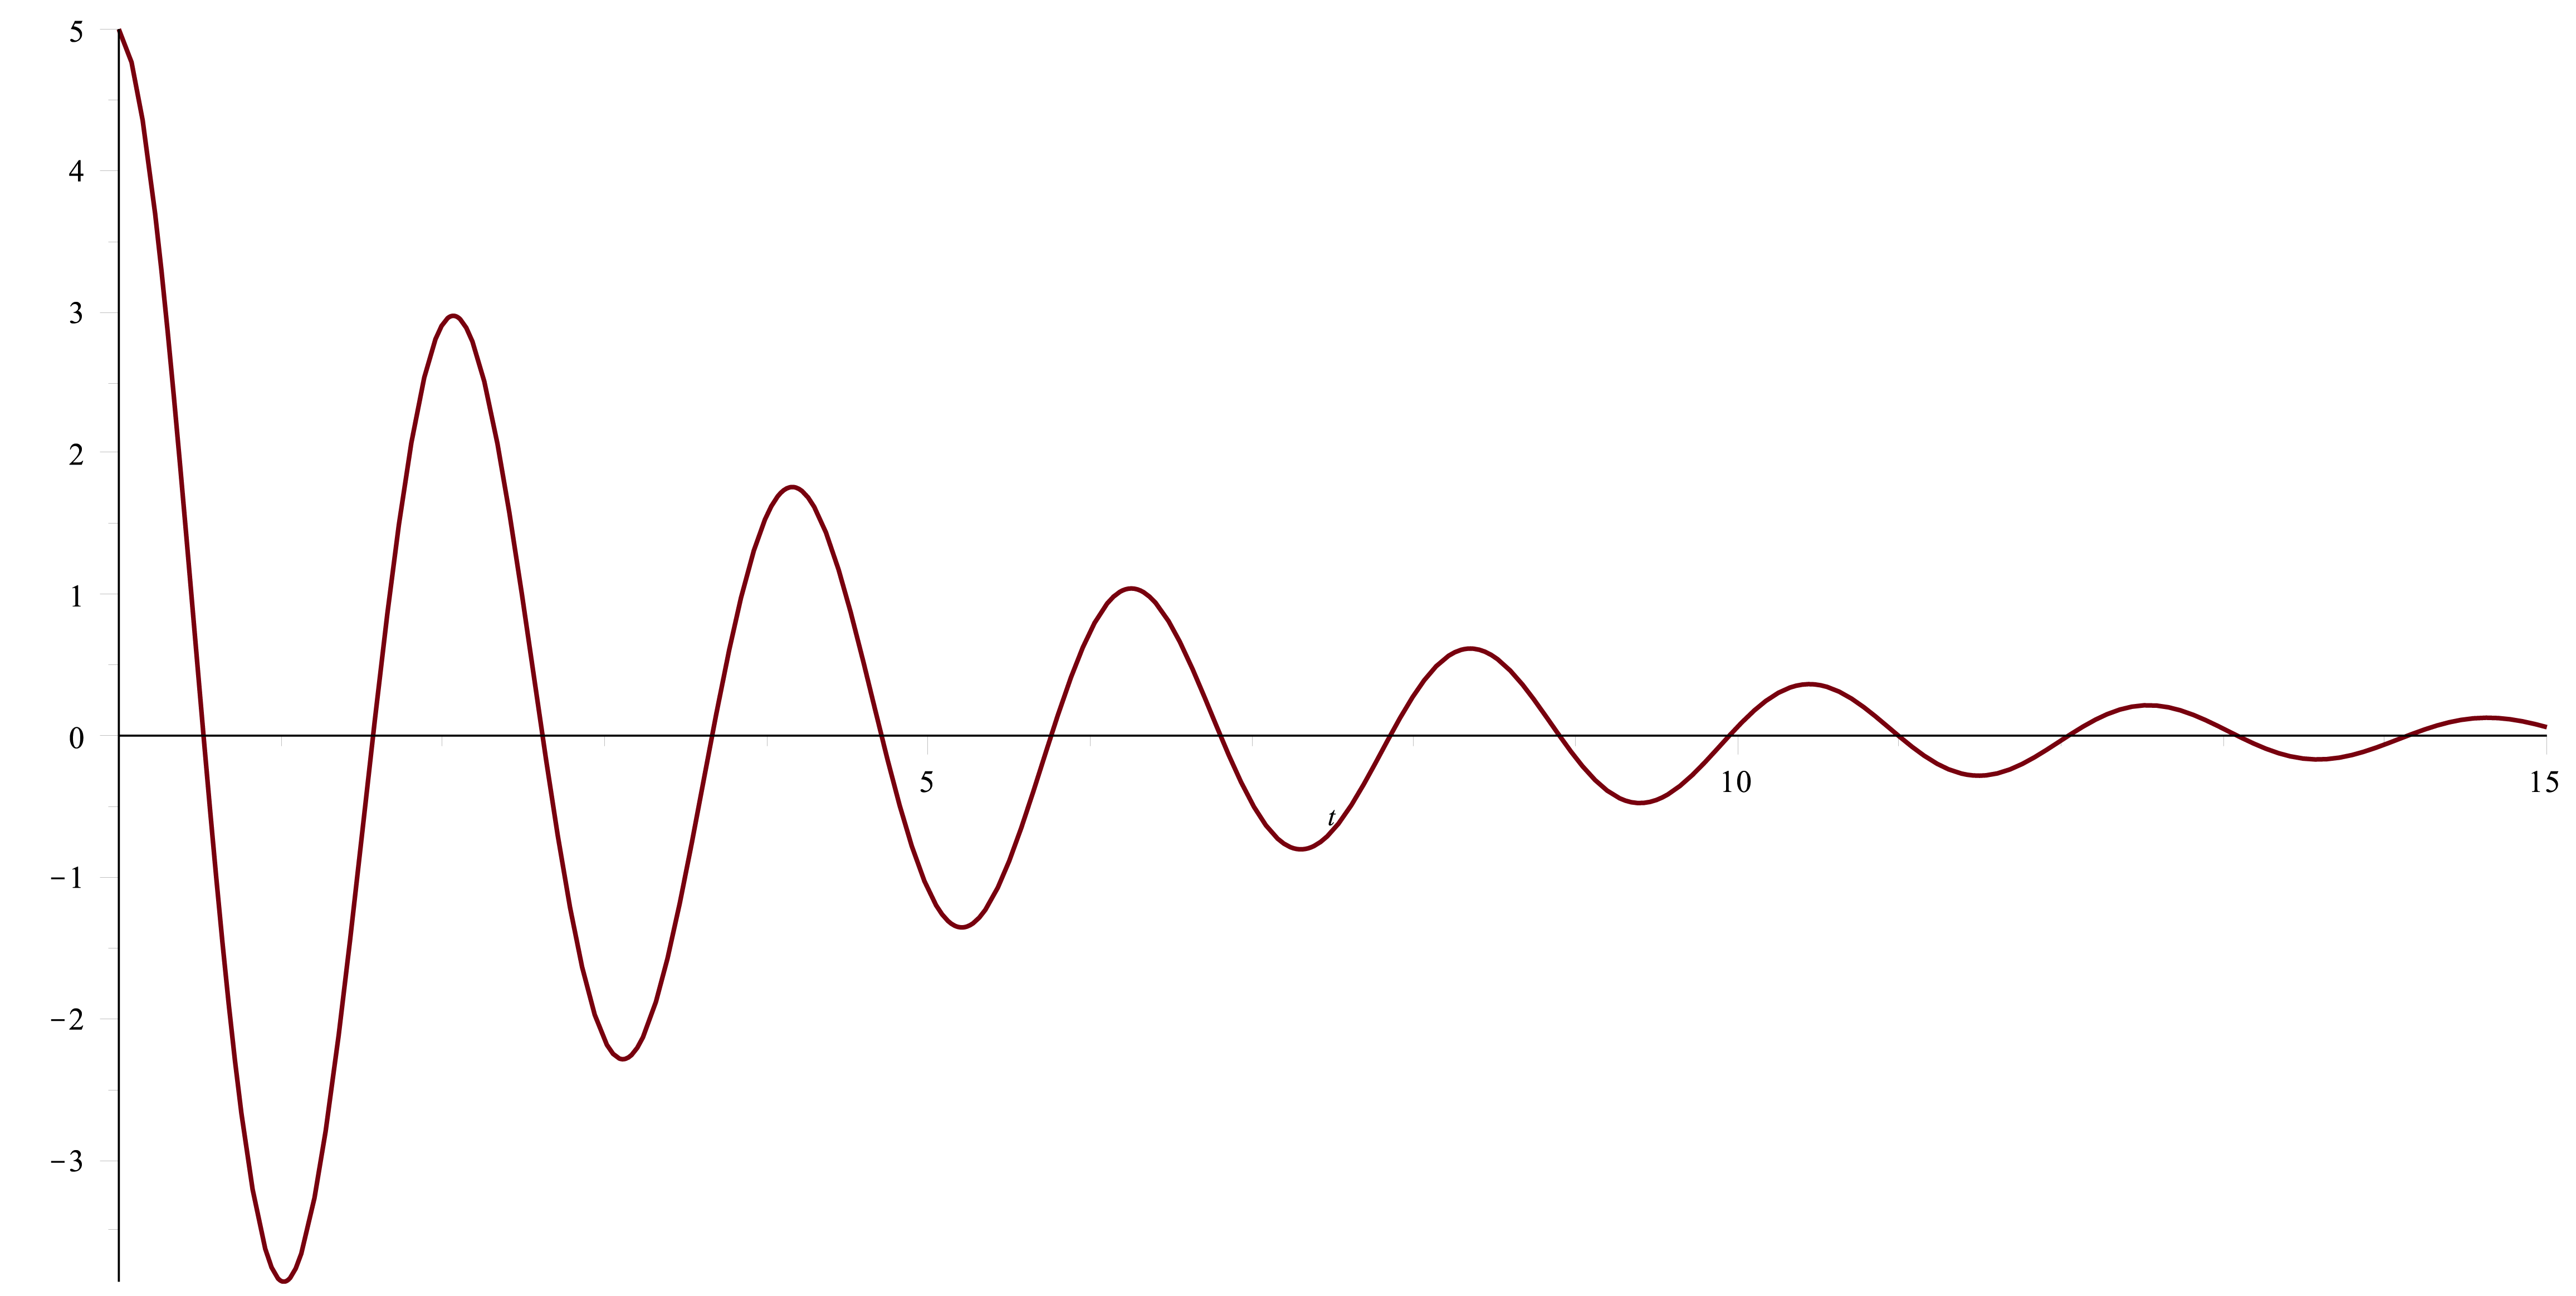
\includegraphics[width=\linewidth]{img/plot}
  \caption{Plot of of f(t) in maple}
  \label{img:function}
\end{figure}

\lipsum[3-4]

\subsection{Page wide figures}
\lipsum[5]

\begin{figure*}[ht]
  \centering
  \includegraphics[width=\linewidth]{img/example2}
  \caption{Another Random cat picture from Google \protect\url{https://static.pexels.com/photos/4067/animal-pet-cute-cat.jpg}}
  \label{img:cat2}
\end{figure*}

\subsection{Formulas and plots}
\lipsum[6]
\begin{figure}[h]
  \centering
  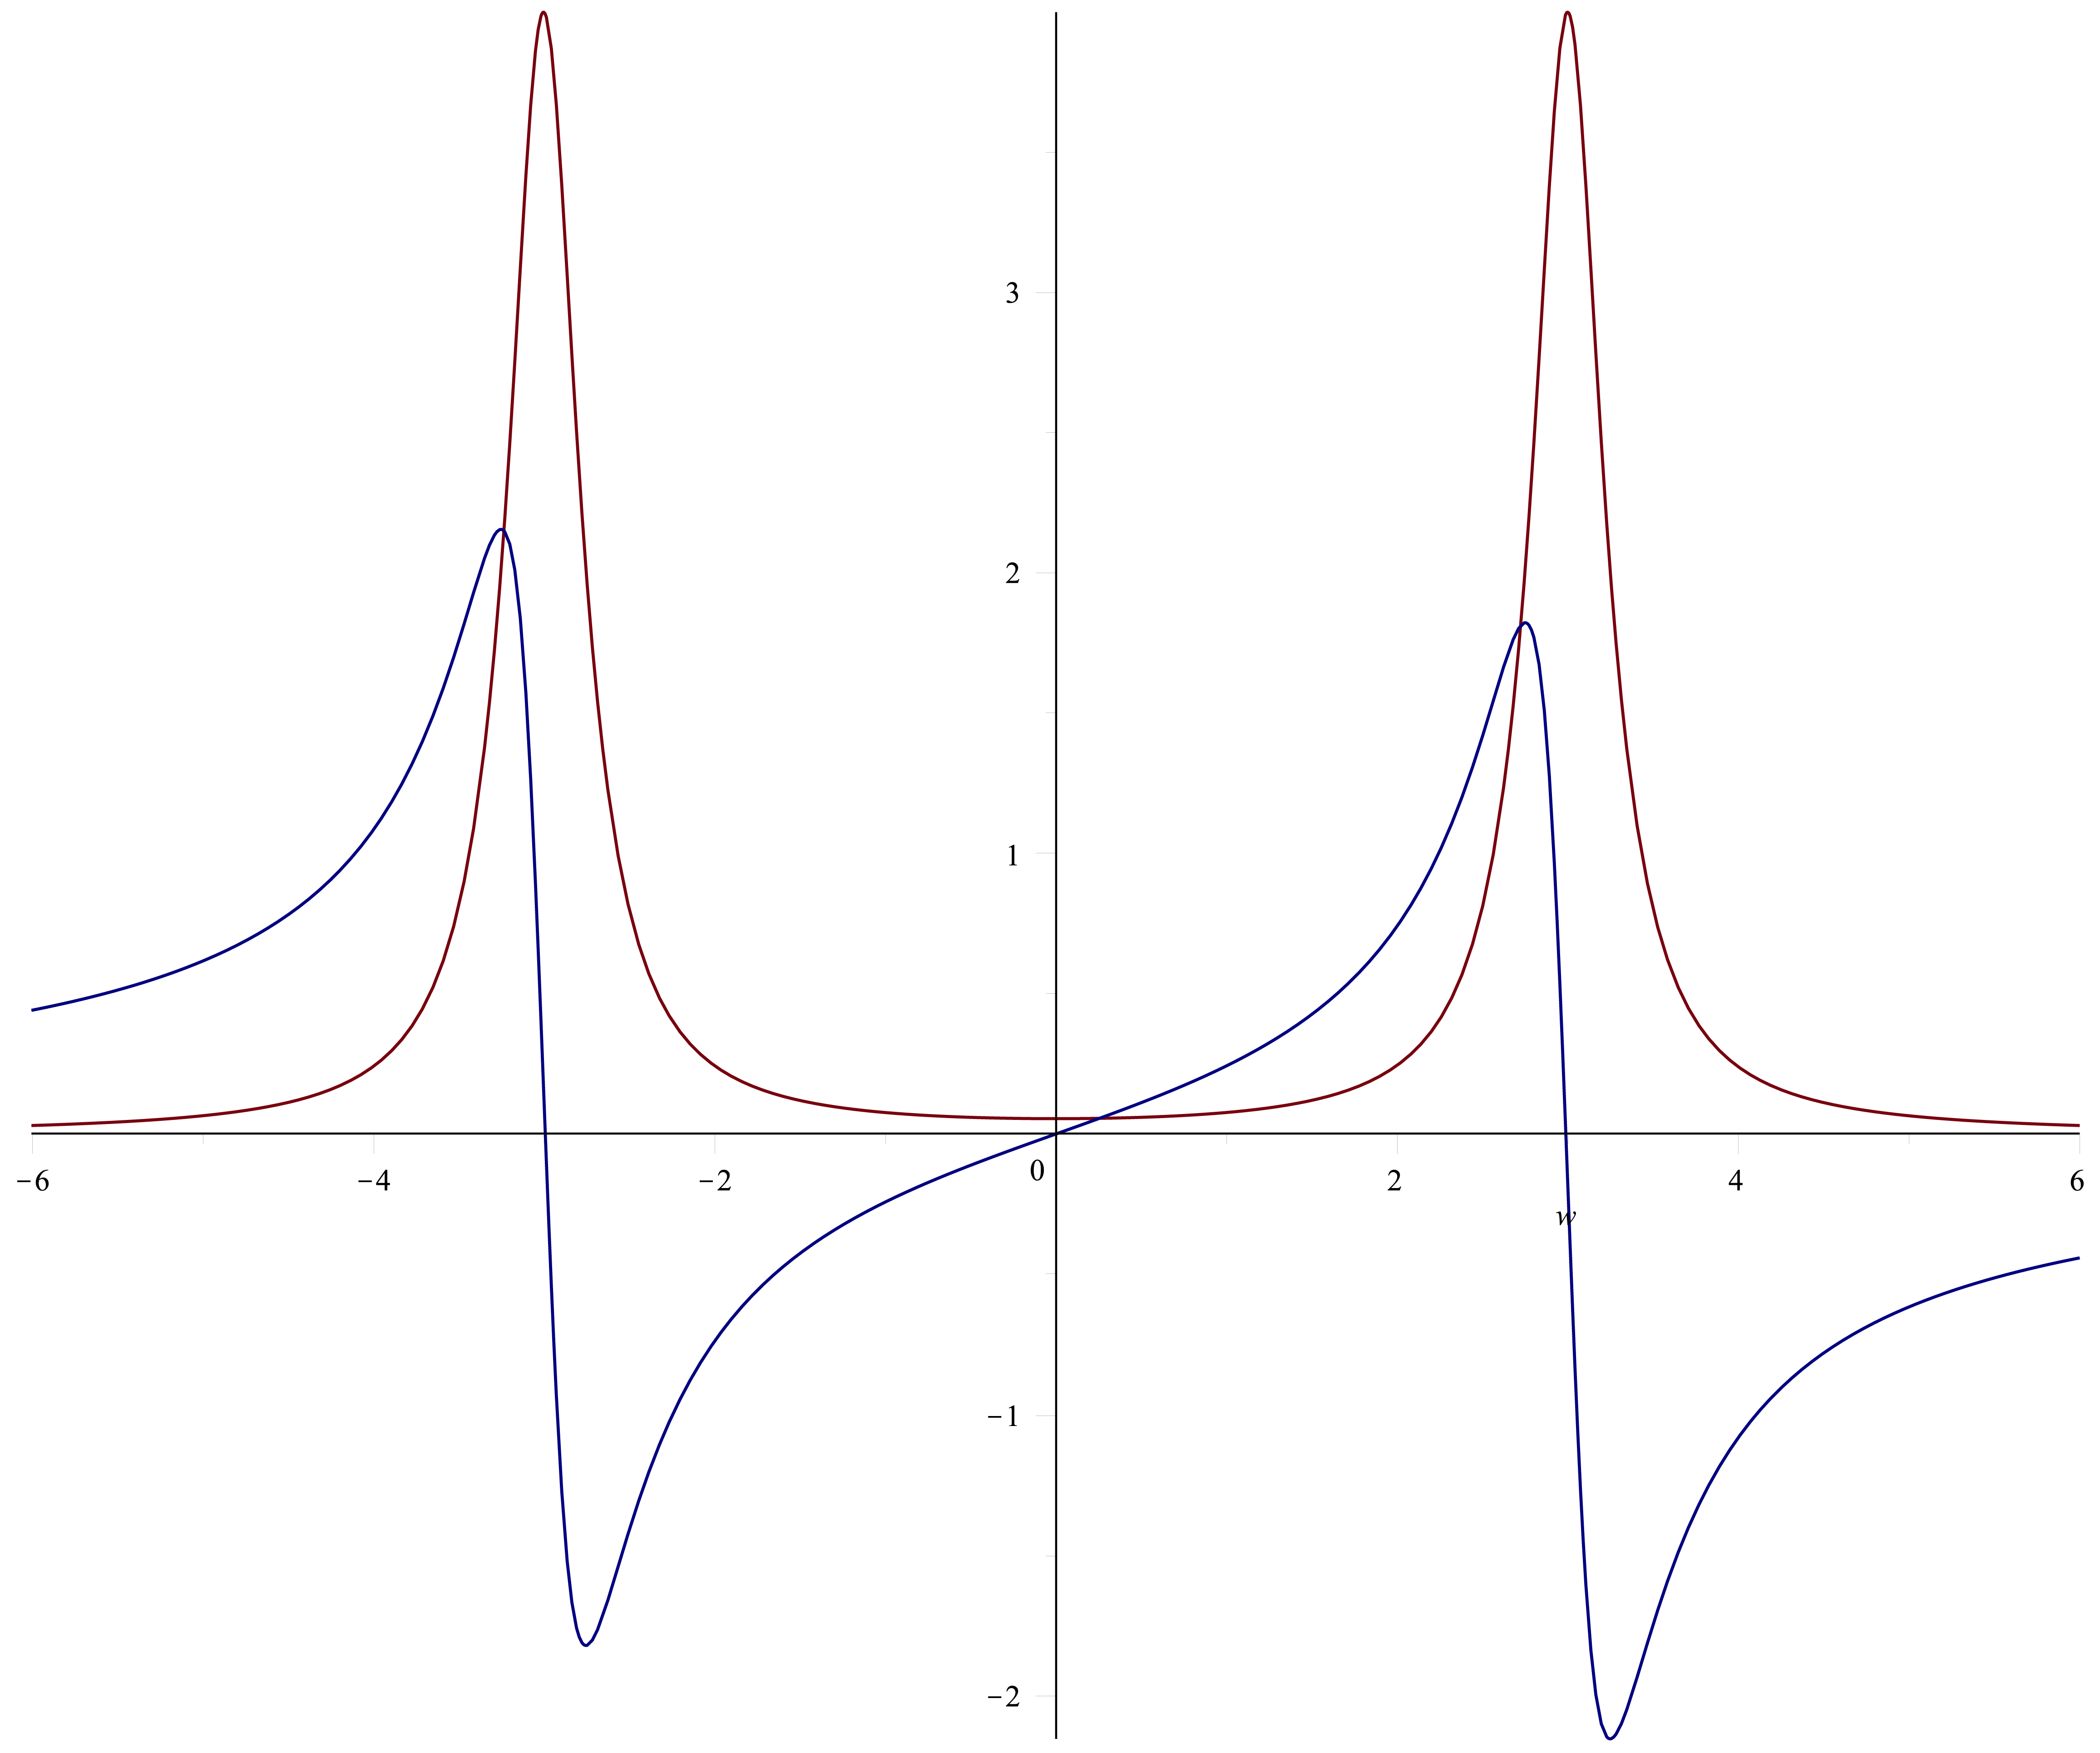
\includegraphics[width=\linewidth]{img/spectrum}
  \caption{Plot of the spectrum of f(t) in maple}
  \label{img:spectrum}
\end{figure}

\begin{align}
    f(t) &= s_0 \cdot e^{-\frac{t}{\tau}} \cdot cos(\omega_s t) \cdot \Theta(t) \nonumber \\
    &= s_0 \cdot e^{-\frac{t}{\tau}} \cdot \frac{1}{2} \Big( e^{i \omega_s t} + e^{-i \omega_s t} \Big) \cdot \Theta(t)\\
    \tilde{f}(\omega) &= \mathcal{F}(f)(\omega) = \frac{1}{\sqrt{2\pi}} \int_{-\infty}^{\infty} f(t) \cdot e^{-i \omega t} dt \nonumber\\
    &= \frac{s_0}{\sqrt{2\pi}} \frac{\frac{1}{\tau} + i \omega}{(\frac{1}{\tau} + i \omega)^2 + \omega_s^2}
\end{align}

\section{Source codes}
\begin{listing}
  \begin{minted}{java}
    public static void main(String[] args) {
      return;
    }
  \end{minted}
  \caption{Standard main method of every java program}
  \label{lst:javamain}
\end{listing}

\lipsum[9-12]

\subsection{Subsection Two.One}
\lipsum[13-14]

  \cite{book:handbook}
  % Input your source files here

  % Bibliography
  \bibliography{bib/bibliography.bib}
\end{document}
